\documentclass[12pt, a4paper]{article}
\input{header.tex}

%% Note that for label to be correct, compile more than 2 times is needed ... %%


%%%%%%%%%%%%%%%Title的資訊%%%%%%%%%%%%%%%
\title{} %標題
\author{} %作者
\date{} %日期

\begin{document}
% \maketitle %製作tilte page
% \thispagestyle{empty}  %去除頁碼
% \thispagestyle{fancy}  %使用fancyhdr
% \tableofcontents %目錄
%%%%%%%%%%%%%%%%%%%include file here%%%%%%%%%%%%%%%%%%%%%%%%%
% 7: 9
\section{5.10}
Consider an n-channel MOSFET with $t_{ox} = \SI{20}\nm$, $\mu_{n} = \SI{650}{\cm\squared\per\V\per\s}$, $V_t = \SI{0.8}\V$ and $W/L = 10$. Find the drain current in the following cases:

\begin{enumerate}[label=(\alph*)]
  \item $v_{GS} = \SI{5}{\V}$ and $v_{DS} = \SI{1}{\V} $\\[5pt]
    \Ans \\
    First we calculate 
    \[ k_n = \mu_n C_{ox} (W / L) = \mu_n \varepsilon_{ox} (W / L) /  t_{ox} \approx \SI{1.12}{\mA\per\V\squared} \]
    Since $v_{GS} > V_t$ and $v_{GS} - v_{DS} = \SI{4}{\V} > V_t$, the MOS is working on the triode region, so 
    \[
      i_D =  k_n \left(v_{GS} - V_t - \frac{1}{2}v_{DS} \right)v_{DS} \approx \SI{4.14}{\mA} 
    \]
  \item $v_{GS} = \SI{2}{\V}$ and $v_{DS} = \SI{1.2}{\V} $\\[5pt]
    \Ans \\
    Now $V_{GS} > V_t$ and $V_{GS} - V_{DS} = \SI{0.8}{\V} = V_t$, the MOS is working on the boundary of the saturation and the triode region, so 
    \[
      i_D = \frac{1}{2} k_n (V_{GS} - V_t)^2 \approx \SI{1.61}{\mA} 
    \]
  \item $v_{GS} = \SI{5}{\V}$ and $v_{DS} = \SI{0.2}{\V} $\\[5pt]
    \Ans \\
    Again $V_{GS} > V_t$ and $V_{GS} - V_{DS} = \SI{4.8}{\V} > V_t$, the MOS is working on the triode region, so 
    \[
      i_D =  k_n \left(v_{GS} - V_t - \frac{1}{2}v_{DS} \right)v_{DS} \approx \SI{0.92}{\mA} 
    \]
  \item $v_{GS} = \SI{5}{\V}$ and $v_{DS} = \SI{5}{\V} $\\[5pt]
    \Ans \\
    Finally since $V_{GS} > V_t$ and $V_{GS} - V_{DS} = \SI{0}{\V} < V_t$, the MOS is working on the saturation region, so 
    \[
      i_D =  \frac{1}{2} k_n (v_{GS} - V_t)^2 \approx \SI{9.88}{\mA} 
    \]
\end{enumerate}
% 18: 23
\section{5.20}
The table below lists 10 different cases labeled (a) to (j) for operating an NMOS transistor with $V_t = \SI{1}{\V} $. In each case the voltages at the source, gate, and drain (relative to the circuit ground) are specified. You are required to complete the tabel entries. Note that if you encounter a case for which $v_{DS}$ is negative, you should exchange the drain and source before solving the problem. You can do this because the MOSFET is a symmetric device.


\Ans \\
\begin{center}
  \begin{tabular}{|l|c|c|c|c|c|c|c|}
    \hline
    & \multicolumn{6}{c|}{Voltage \si\V} & \\ \cline{2-7}
    Case & $V_S$ & $V_G$ & $V_D$ & $V_{GS}$ & $V_{OV}$ & $V_{DS} & Region of operation \\
    \hline
    a & $+1.0$ & $+1.0$ & $+2.0$ & $0$ & $0$ & $1.0$ & Cut-off \\
    b & $+1.0$ & $+2.5$ & $+2.0$ & $1.5$ & $0.5$ & $1.0$ & Saturation \\
    c & $+1.0$ & $+2.5$ & $+1.5$ & $1.5$ & $0.5$ & $0.5$ & Boundary of Sat./Tri. \\
    d & $+1.0$ & $+1.5$ & $+2.0$ & $0.5$ & $0$ & $1.0$ & Cut-off \\
    e & $0$ & $+2.5$ & $+1.0$ & $2.5$ & $1.5$ & $1$ & Triode \\
    f & $+1.0$ & $+1.0$ & $+1.0$ & $0$ & $0$ & $0$ & Cut-off \\
    g & $-1.0$ & $0$ & $0$ & $1.0$ & $0$ & $1.0$ & Boundary of Cut./Sat. \\
    h & $-1.5$ & $0$ & $0$ & $1.5$ & $0.5$ & $1.5$ & Saturation \\
    i & $-1.0$ & $0$ & $+1.0$ & $1.0$ & $0$ & $2.0$ & Saturation \\
    j & $+0.5$ & $+2.0$ & $+0.5$ & $1.5$ & $0.5$ & $0$ & Triode \\
    \hline
  \end{tabular}
\end{center}

\clearpage
% 21: 26
\section{3.21}
For the circuit shown in Fig.~\ref{fig:3.21}, both diodes are identical,
conducting \SI{10}{\mA} at \SI{0.7}{\V} and \SI{100}{\mA}
at \SI{0.8}{\V}. Find the value of $R$ for which $V = \SI{80}{\mV}$.

\begin{figure}[H]
  \centering
  \begin{circuitikz}
    \draw[color=black, thick] (0, 0) to [I, l=10<\mA>, *-*]
      ++ (0, -2.5) node[](n1){} to [Do, l_=$D_2$] ++(0, -1.5) node[ground] {}
    (n1) to[short, i={\color{blue} $i_1$}] ++(1.5, 0)
    to [Do, -*, l^=$D_1$] ++(0, -1.5) node[](n2){}
    to [R, l_=$R$] ++(0, -2.5) node[ground]{} 
    (n2) to [short, -o] ++(1, 0) to [open, v^={\color{red} $V$}] ++(0, -3)
    ;
  \end{circuitikz}
  \caption{}
  \label{fig:3.21}
\end{figure}

\Ans \\
Model the diode as $i = I_s \ex^{V / V_T}$ and solve $I_S, V_T$ with
$(i, V) = (\SI{10}{\mA}, \SI{0.7}{\V}), (\SI{100}{\mA}, \SI{0.8}{\V})$.
We have
\[
\frac{i_2}{i_1} = 10 = \ex^{\frac{V_2 - V_1}{V_T}} \; \Rightarrow \;
V_T = \frac{V_2 - V_1}{ \log 10 } = \SI{43.4}\mV \]
and thus $I_S = \SI{1e-6}{\mA}$. So
\begin{align*}
  & V_{D_2} - V_{D_1} = V \\
  \Leftrightarrow \; &V_T \log \frac{i_2}{i_1} = V \\
  \Leftrightarrow \; &V_T \log \frac{\SI{10}{\mA} - i_1}{i_1} = \SI{80}{\mV} \\
  \Leftrightarrow \; &i_1 \approx \SI{1.367}{\mA}
\end{align*}
Finally $R = V / i_1 \approx \SI{80}{\mV} / \SI{1.367}{\mA} = \SI{58.5}{\ohm}$.

% 38: 46
\section{3.38}
In the circuit shown in Fig.~\ref{fig:3.38}, $I$ is a dc current and
$v_s$ is a sinusoidal signal. Capacitors $C_1$ and $C_2$ are very large;
their function is to couple the signal to and from the diode but block the
dc current from flowing into the signal source or the load (not shown).
Use the diode small-signal model to show that the signal component of the
output voltage is
\[ v_o = v_s \frac{V_T}{V_T + IR_s} \]
If $v_s = \SI{10}{\mV}$, find $v_o$ for $I = \SI{1}{\mA}, \SI{0.1}{\mA}$, and
\SI{1}{\uA}. Let $R_s = \SI{1}{\kohm}$. Assume $n = 2$. At
what value of $I$ does $v_o$ become one-half of $v_s$?
Note that this circuit functions as a signal attenuator with the
attenuation factor controlled by the value of the dc current $I$.

\begin{figure}[H]
  \centering
  \begin{circuitikz}[>=triangle 45, scale=0.8, transform shape]
    \draw[color=black, thick] (0, 0) node[ground]{}
      to [V, l=$v_s$] (0, 3) to [R, l=$R_s$] (3, 3)
      to [C, l=$C_1$, o-*] (6, 3) node[](n1){} to [C, l=$C_2$, -o] (9, 3)
      to [open, v^=$v_o$] (9, -0.5)
      (n1) to [Do] (6, 0) node[ground]{}
      (6, 6) node[](Iout){} to [I, l=$I$] (n1)
      ;
    \draw[color=black, thick, ->]
      (6, 5) to (6, 6.5)
      ;
  \end{circuitikz}
  \caption{}
  \label{fig:3.38}
\end{figure}

\Ans \\
Notice that there is no dc current flow between the source
and load. Thus we can model diode as a resistor for small signal: \footnote{differentiate $I = I_s e^{v/v_T}$}
\[ r_d = \frac{V_T}{I} \]
And for small ac signal, since $C_1, C_2$ are large, $Z = 1 / (\img \omega C)$
are small, we can treat $C_1, C_2$ as short. So we have
\[ \frac{v_s}{R_s + r_d} = \frac{v_o}{r_d} \; \Rightarrow \;
v_o = v_s\frac{V_T}{V_T + IR_s} \]
as desired. Plug in the values, we get $v_o(I = \SI{1}\mA) = \SI{0.24}\uV$, $v_o(I = \SI{0.1}\mA) = \SI{2}\mV$ and $v_o(I = \SI{1}\uA) = \SI{9.62}\mV$.
If now we assume $n = 2$, what we only need is to substitute $V_T \rightarrow n V_T = 2 V_T$. So the formula becomes 
\[ v_o = v_s\frac{2V_T}{2V_T + IR_s} \] and hence for $v_o = v_s \ 2, nV_T = IR_s \Rightarrow I = 2 (\SI{25}\mV) / (\SI{1}\kohm) =  \SI{50}\uA$.

% 40: 48
\section{3.40}
In the capacitor-coupled attenuator circuit shown in Fig.~\ref{fig:3.40},
$I$ is a dc current that varies from \SI{0}{\mA} to
\SI{1}{\mA}, and $C_1$ and $C_2$ are large coupling capacitors.
For very small input signals, so that the diodes can be represented by
their small-signal resistances $r_{d1}$ and $r_{d2}$, show that
$\dfrac{v_o}{v_i} = \dfrac{r_{d2}}{r_{d1}+r_{d2}}$ and hence
that $\dfrac{v_o}{v_i}  = I$, where $I$ is in
\si{\mA}. Find $v_o/v_i$ for $I = \SI{0}{\uA}, \SI{1}{\uA},
\SI{10}{\uA}, \SI{100}{\uA}, \SI{500}{\uA}, \SI{600}{\uA},
\SI{900}{\uA}, \SI{990}{\uA}, \SI{1}{\mA}$. \footnote{Seriously ??}

\begin{figure}[H]
  \centering
  \begin{circuitikz}[>=triangle 45]
    \draw[color=black, thick] (0, 0) node[left](vi){$v_i$}
      to [C, l=$C_1$, o-*] (2, 0) node[](n1){} to [I, l=$I$] (2, -2)
      (6, 2) node[right](vo){$v_o$} to [C, l_=$C_2$, o-*] (4, 2)
      to [Do, l=$D_2$, i={\color{blue} $I_2$}] (4, 0) node[ground]{}
      (3, 4) to [I, l=$\SI{1}{\mA}$, -*] (3, 2) -- (2, 2)
      to [Do, l=$D_1$] (n1)
      (3, 2) -- (4, 2)
      ;
    \draw[color=black, thick, ->]
      (2, -1) -- (2, -2.5)
      ;
    \draw[color=black, thick, ->]
      (3, 3.5) -- (3, 4.5)
      ;
  \end{circuitikz}
  \caption{}
  \label{fig:3.40}
\end{figure}

\Ans \\
Again since $v_i, v_o$ is block by the capasitor, no current flow to the middle part, so $I_2 = \SI{1}\mA - I$, and \[ r_{d1} = \frac{V_T}{I}, \; r_{d2} = \frac{V_T}{I_2} = \frac{V_T}{\SI{1}\mA - I} \]
and so
\[ 
  \frac{r_{d1}}{r_{d2}} = \frac{I_2}{I} 
\]
Now for small AC signal, since $C_1, C_2$ large, we could assume $C_1, C_2$ to be short, and hence $D_1, D_2$ are in series with $v_i$, thus
\[
  \frac{v_o}{v_i} = \frac{r_{d2}}{r_{d2} + r_{d1}} = \frac{I}{I+I_2} = \frac{I}{\SI{1}\mA}
\]
\si{\mA}. For $I = \SI{0}{\uA}, \SI{1}{\uA},
\SI{10}{\uA}, \SI{100}{\uA}, \SI{500}{\uA}, \SI{600}{\uA},
\SI{900}{\uA}, \SI{990}{\uA}, \SI{1}{\mA}$, $v_o / v_i = 0, 10^{-3}, 10^{-2}, 0.1, 0.5, 0.6, 0.9, 0.99, 1$.


% 45: 53
\section{3.45}
Consider the voltage-regulator circuit shown in Fig.~\ref{fig:3.45} under the
condition that a load current $I_L$ is drawn from the output terminal.
\begin{enumerate}[(a)]
  \item If the value of $I_L$ is sufficiently small that the
    corresponding change in regulator output voltage $\Delta V_O$ is
    small enough to justify using the diode small-signal model, show
    that
    \[ \frac{\Delta V_O}{I_L} = -(r_d \parallel R) \]
    This quantity is known as the load regulation and is usually
    expressed in \si{\mV/\mA}.
  \item If the value of $R$ is selected such that at no load the voltage
    across the diode is \SI{0.7}{\V} and the diode current is $I_D$,
    show that the expression derived in (a) becomes
    \[ \frac{\Delta V_O}{I_L} =
      -\frac{nV_T}{I_D}\frac{V^+ -0.7}{V^+ - 0.7 + nV_T} \]
    Select the lowest possible value for $I_D$ that results in a load
    regulation $\le \SI{5}{\mV/\mA}$. Assume $n = 2$.
    If $V^+$ is nominally \SI{10}{\V}, what value of $R$ is required?
    Also, specify the diode required in terms of its $I_S$.
  \item Generalize the expression derived in (b) for the case of $m$
    diodes connected in series and $R$ adjusted to obtain $V_O =
    0.7m\si{\V}$ at no load.
\end{enumerate}

\begin{figure}[H]
  \centering
  \begin{circuitikz}[>=triangle 45]
    \draw[color=black, thick] (0, 0) to [R, l=$R$] (0, -3) node[](n1){}
      to [Do] (0, -6) node[ground]{}
      (n1) to[short, *-o] (3, -3) to [open, v^=$V_o$] (3, -6.5)
      ;
    \draw[color=black, thick, ->]
      (0, -1) -- (0, 0.5) node[above](vp){$V^+$}
      ;
  \end{circuitikz}
  \caption{}
  \label{fig:3.45}
\end{figure}

\begin{enumerate}[(a)]
  \item \Ans \\
    We could model the diode as a voltage source $v_d$ in series with
    a resistor $r_d$ in small signal. The circuit is now a linear circuit
    and we could use supercomposition to turn off $V^+$ and $v_d$, so now
    $R$ is parellel with $r_d$, and hence 
    $\Delta V_o / I_L = -(R \parallel r_d)$.
    (Note: the direction of $I_L$ is reversed.)
  \item \Ans \\
    Notice now we have
    \begin{align*}
      R &= \frac{V^+ - 0.7}{I_D} \\
      r_d &= \frac{nV_T}{I_D} \\
      -(R \parallel r_d) &= -\frac{nV_T}{I_D} \frac{V^+ - 0.7}{V^+ - 0.7 + nV_T }
    \end{align*}
    We plug in the requirements and solve for $I_D$ and get
    $I_D \approx \SI{9.95}\mA$, so $R = V^+ - 0.7 / I_D \approx \SI{935}\ohm$.
    $I_S = I_D \ex^{-0.7/(nV_T)} \approx \SI{8.27e-9}\A$.
  \item \Ans \\
    Now $\Delta V_O / I_L = -(R \parallel m r_d)$ and
    $R = (V^+ - 0.7m) / I_D$, $r_d$ remains unchanged, so 
    \[
      \frac{\Delta V_O}{I_L} = -(R \parallel m r_d) =
      -\frac{mnV_T}{I_D} \frac{V^+ - 0.7m}{V^+ - 0.7m + mnV_T }
    \]
\end{enumerate}

% 48: 56
\section{3.48}
A particular design of a voltage regulator is shown in Fig.~\ref{fig:3.48}.
Diodes $D_1$ and $D_2$ are 10-\si{\mA} units; that is,
each has a voltage drop of \SI{0.7}{\V} at a current of
\SI{10}{\mA}. Use the diode exponential model and iterative
analysis to answer the follwing questions:
\begin{enumerate}[(a)]
  \item What is the regulator output voltage $V_O$ with the
    150-\si{\ohm} load connected?
  \item Find $V_O$ with no load.
  \item With the load connected, to what value can the 5-\si{\V}
    supply be lowered while maintaining the loaded output voltage
    within \SI{0.1}{\V} of its nominal value?
  \item What does the loaded output voltage become when the 5-\si{\V}
    supply is raised by the same amount as the drop found in (c)?
  \item For the range of changes explored in (c) and (d), by what
    percentage does the output voltage change for each percentage
    change of supply voltage in the worst case?
\end{enumerate}

\begin{figure}[H]
  \centering
  \begin{circuitikz}[>=triangle 45]
    \draw[color=black, thick] (0, 0) to [R, l=180<\ohm>] (0, -3) node[](n1){}
      -- (0, -3.3) to [Do, l_=$D_1$] (0, -4.5) to [Do, l_=$D_2$] (0, -5.8)
      -- (0, -6) node[ground]{}
      (n1) to[short, *-o] (1.5, -3) -| (3, -3)
      to [R, l=$\SI{150}{\ohm}$] (3, -6) node[ground]{}
      (1.2, -3) to[open, v^=$V_o$] (1.2, -6.5)
      (n1) node[left]{\color{blue} $n_1$}
      ;
    \draw[color=black, thick, ->]
      (0, -1) -- (0, 0.5) node[above](vp){$+\SI{5}\V$}
      ;
  \end{circuitikz}
  \caption{}
  \label{fig:3.48}
\end{figure}

\begin{enumerate}[(a)]
  \item \Ans \\
    \[ I_S = (\SI{10}\mA) \ex^{-0.7 / V_T} \approx \SI{6.9e-15}\A \]
    We use the nodal analysis at $n_1$. Since the voltage across a diode is $V_O / 2$, we get
    \begin{align*}
      I_S \ex^{V_O/(2V_T)} &= \frac{\SI{5}\V}{\SI{180}\ohm} -
      (1 / (\SI{180}\ohm) + 1 / (\SI{150}\ohm)) V_O \\
                        &= \SI{27.8}\mA - (\SI{12.2}\mohm) V_O
    \end{align*}

    We begin the iterate at $(v, i) = (0, 0)$ and obtain
    \[
      (0, 0) \rightarrow (0, 0.0278) \rightarrow (1.451, 0.0278) \rightarrow
      (1.451, 0.010) \rightarrow (1.401, 0.011) 
    \]
    and thus $V_O \approx 1.401$. (Which the real answer is about $1.403$)
  \item \Ans \\
    Similarly, $(5 - V_O) / 180 = I_S \ex^{V_O / (2V_T)}$. Solve for $V_O$
    and we get $V_O \approx \SI{1.434}\V$.
  \item \Ans \\
    We lower $V_O$ to $V_O' \approx 1.303$ and get
    \[
      V' = 180 \left( I_S \ex^{V_O' / (2V_T)} +
        \frac{V'_O }{150} \right) + V_O' \approx \SI{3.125}{\V}
    \]
  \item \Ans \\
      $V'' = V + (V - V') = \SI{6.875}\V $, and again solve for $V_O$ we get $V_O \approx \SI{1.436}\V$.
  \item \Ans \\
    \begin{align*}
      \%\text{Worst}  &= 100\% \cdot \frac{5}{5 - 3.125} \max \left( \abs*{\frac{1.303 - 1.403}{1.403}} , \abs*{\frac{1.436-1.403}{1.403}} \right) \\
      &\approx 19\%
    \end{align*}
    
\end{enumerate}

% 52: 61
\section{3.52}
Design a 7.5-\si{\V} zener regulator circuit using a 7.5-\si{\V}
zener specified at \SI{12}{\mA}. The zener has an incremental
resistance $r_z = \SI{30}{\ohm}$ and a knee current of \SI{0.5}{\mA}.
The regulator operates from a 10-\si{\V} supply and has a
1.2-\si{\kohm} load. What is the value of $R$ you have chosen?
What is the regulator output voltage when the supply is \SI{10}{\percent}
high? Is \SI{10}{\percent} low? What is the output voltage when both the
supply is \SI{10}{\percent} high and the load is removed? What is
the smallest possible load resistor that can be ued while the zener
operates at a current no lower than the knee current while the supply
is \SI{10}{\percent} low? What is the load voltage in this case?

\Ans \\
First calculate $V_{Z0} = V_Z - r_z I_Z = \SI{7.14}{\V}$. Now we need to
choose a value of $R$ such that the current $I_D$ flowing into the zener diode
is not smaller that the knee current of that diode. We have
$V_O = I_Dr_z + V_{Z0}$, so
\[
  \left((1/(\SI{1.2}{\kohm}) + (1/R)\right) V_O + I_D - 10/R = 0
    \quad \text{and} \quad I_D \ge \SI{0.5}{\mA}.
\]
We choose $R = \SI{200}{\ohm}$ as an example.
Now we obtain the equality:
\[ \left((1/R_L) + (1/r_z) + (1/R)\right)V_O = V_S/R + V_{Z0}/r_z \]
where $R_L$ is the load resistance, $V_S$ is the supply voltage. \\
When the supply is \SI{10}{\percent} high, $V_O \approx \SI{7.48}{\V}$. \\
When the supply is \SI{10}{\percent} low, $V_O \approx \SI{7.23}{\V}$. \\
If supply is \SI{10}{\percent} high and load resistor is removed,
then $R_L = \infty$, $V_O \approx \SI{7.64}{\V}$.
Since $I_D = (V_O - V_{Z0})/r_z$ must greater that \SI{0.5}{\mA}, we have
$V_O \ge \SI{7.155}{\V}$. So the smallest value of $R_L$ when supply is
\SI{10}{\percent} low is \SI{561}{\ohm} approximately. And the load voltage
is equal to $V_O \approx \SI{7.155}{\V}$.

% 53: 63
\section{3.53}
A zener shunt regulator employ a 9.1-\si{\V} zener diode for which
$V_Z = \SI{9.1}{\V}$ at $I_Z = \SI{9}{\mA}$, with $r_z = \SI{30}{\ohm}$
and $I_{ZK}=\SI{0.3}{\mA}$. The available supply voltage of \SI{15}{\V}
can vary as much as $\pm\SI{10}{\percent}$.
\begin{enumerate}[(a)]
  \item For this diode, what is the value of $V_{Z0}$?
  \item For a nominal load resistance $R_L$ of \SI{1}{\kohm}
and a nominal zener current of \SI{10}{\mA}, what current must flow
in the supply resistor $R$?
  \item For the nominal value of supply voltage, select a value for resistor $R$, specified to one significant digit, to provide at least that current. What nominal output voltage results?
  \item For a $\pm\SI{10}{\percent}$ change in the supply voltage, what variation
in output voltage results?
  \item If the load current is reduced by
\SI{50}{\percent}, what increase in $V_O$ results?
  \item What is the smallest value of load resistance that can be tolerated while maintaining
regulation when the supply voltage is low?  What is the lowest possible output voltage that results? 
  \item Calculate values for the line regulation
and for the load regulation for this circuit using the numerical results
obtained in this problem.
\end{enumerate}

\Ans \\
\begin{enumerate}[(a)]
  \item $V_{Z0} = V_Z - r_z I_Z = \SI{8.83}{\V}$.
  \item If nominal zener current is \SI{10}{\mA}, then $V_O = V_{Z0} + \SI{10}{\mA} \cdot r_z = \SI{9.13}{\V}$.
So the current flowing into $R$ is equal to $V_O/R_L + \SI{10}{\mA} =
\SI{19.13}{\mA}$.
  \item Since $(V_S - V_O)/R \ge \SI{19.13}{\mA}$,
$R \le \SI{306.8}{\ohm} \Rightarrow R \approx \SI{300}{\ohm}$. And we have
$V_O \approx \SI{9.14}{\V}$ when $R = \SI{300}{\ohm}$. 
  \item When $V_S$ is \SI{10}{\percent} high, $V_O \approx \SI{9.27}{\V}$. When $V_S$ is \SI{10}{\percent} low, $V_O \approx \SI{9.01}{\V}$.
  \item If load current is reduced by \SI{50}{\percent}, then we have load current
$I_L = \SI{4.57}{\mA}$. Thus
\[ \frac{V_S - V_O}{R} = I_L + \frac{V_O - V_{Z0}}{r_z}
  \; \Rightarrow \; V_O \approx \SI{9.27}{\V}. \]
  \item The load resistance should not be too small so that $I_D$ is smaller than
$I_{ZK}$. So we can obtain the inequality:
\[ \frac{V_O - V_{Z0}}{r_z} \ge I_{ZK} \; \Rightarrow \;
V_O \ge \SI{8.839}{\V}, R_L \ge \SI{436.8}{\ohm}. \]
\item Line regulation: $\Delta V_O/ \Delta V_S \approx \SI{8.67}{\percent}$. \\
Load regulation: $\Delta V_O/I_L \approx \SI{-27.3}{\mV/\mA}$.
\end{enumerate}

% 60: 74
\section{3.60}
The circuit in Fig.~\ref{fig:3.60} implements a complementary-output
rectifier. Sketch and clearly label the waveforms of $v_O^+$ and $v_O^-$.
Assume a 0.7-\si{\V} drop across each conducting diode. If the
magnitude of the average of each output is to be \SI{15}{\V}, find
the required amplitude of the sine wave across the entire secondary
winding. What is the PIV of each diode?

\begin{figure}[H]
  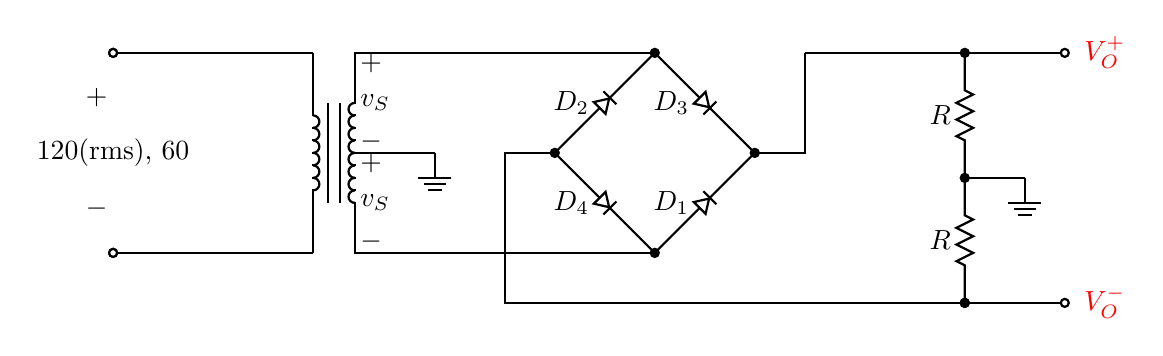
\begin{tikzpicture}[scale=2.54]
% dpic version 2014.Jan.01 option -g for TikZ and PGF 1.01
\ifx\dpiclw\undefined\newdimen\dpiclw\fi
\global\def\dpicdraw{\draw[line width=\dpiclw]}
\global\def\dpicstop{;}
\dpiclw=0.8bp
\dpiclw=0.8bp
\dpicdraw[fill=white](0,0) circle (0.007874in)\dpicstop
\dpicdraw (0,0)
 --(1,0)\dpicstop
\dpicdraw (1,0)
 --(1,-0.3125)\dpicstop
\dpicdraw (1,-0.3125)
 --(0.994444,-0.3125)\dpicstop
\dpicdraw (1,-0.3125)
 ..controls (1.017259,-0.3125) and (1.03125,-0.326491)
 ..(1.03125,-0.34375)
 ..controls (1.03125,-0.361009) and (1.017259,-0.375)
 ..(1,-0.375)\dpicstop
\dpicdraw (1,-0.375)
 --(0.994444,-0.375)\dpicstop
\dpicdraw (1,-0.375)
 ..controls (1.017259,-0.375) and (1.03125,-0.388991)
 ..(1.03125,-0.40625)
 ..controls (1.03125,-0.423509) and (1.017259,-0.4375)
 ..(1,-0.4375)\dpicstop
\dpicdraw (1,-0.4375)
 --(0.994444,-0.4375)\dpicstop
\dpicdraw (1,-0.4375)
 ..controls (1.017259,-0.4375) and (1.03125,-0.451491)
 ..(1.03125,-0.46875)
 ..controls (1.03125,-0.486009) and (1.017259,-0.5)
 ..(1,-0.5)\dpicstop
\dpicdraw (1,-0.5)
 --(0.994444,-0.5)\dpicstop
\dpicdraw (1,-0.5)
 ..controls (1.017259,-0.5) and (1.03125,-0.513991)
 ..(1.03125,-0.53125)
 ..controls (1.03125,-0.548509) and (1.017259,-0.5625)
 ..(1,-0.5625)\dpicstop
\dpicdraw (1,-0.5625)
 --(0.994444,-0.5625)\dpicstop
\dpicdraw (1,-0.5625)
 ..controls (1.017259,-0.5625) and (1.03125,-0.576491)
 ..(1.03125,-0.59375)
 ..controls (1.03125,-0.611009) and (1.017259,-0.625)
 ..(1,-0.625)\dpicstop
\dpicdraw (1,-0.625)
 --(0.994444,-0.625)\dpicstop
\dpicdraw (1,-0.625)
 ..controls (1.017259,-0.625) and (1.03125,-0.638991)
 ..(1.03125,-0.65625)
 ..controls (1.03125,-0.673509) and (1.017259,-0.6875)
 ..(1,-0.6875)\dpicstop
\dpicdraw (1,-0.6875)
 --(0.994444,-0.6875)\dpicstop
\dpicdraw (1,-0.6875)
 --(1,-1)\dpicstop
\dpicdraw (1.072917,-0.25)
 --(1.072917,-0.75)\dpicstop
\dpicdraw (1.135417,-0.25)
 --(1.135417,-0.75)\dpicstop
\dpicdraw (1.208333,-0.75)
 --(1.208333,-0.75)\dpicstop
\dpicdraw (1.208333,-0.75)
 --(1.213889,-0.75)\dpicstop
\dpicdraw (1.208333,-0.75)
 ..controls (1.191074,-0.75) and (1.177083,-0.736009)
 ..(1.177083,-0.71875)
 ..controls (1.177083,-0.701491) and (1.191074,-0.6875)
 ..(1.208333,-0.6875)\dpicstop
\dpicdraw (1.208333,-0.6875)
 --(1.213889,-0.6875)\dpicstop
\dpicdraw (1.208333,-0.6875)
 ..controls (1.191074,-0.6875) and (1.177083,-0.673509)
 ..(1.177083,-0.65625)
 ..controls (1.177083,-0.638991) and (1.191074,-0.625)
 ..(1.208333,-0.625)\dpicstop
\dpicdraw (1.208333,-0.625)
 --(1.213889,-0.625)\dpicstop
\dpicdraw (1.208333,-0.625)
 ..controls (1.191074,-0.625) and (1.177083,-0.611009)
 ..(1.177083,-0.59375)
 ..controls (1.177083,-0.576491) and (1.191074,-0.5625)
 ..(1.208333,-0.5625)\dpicstop
\dpicdraw (1.208333,-0.5625)
 --(1.213889,-0.5625)\dpicstop
\dpicdraw (1.208333,-0.5625)
 ..controls (1.191074,-0.5625) and (1.177083,-0.548509)
 ..(1.177083,-0.53125)
 ..controls (1.177083,-0.513991) and (1.191074,-0.5)
 ..(1.208333,-0.5)\dpicstop
\dpicdraw (1.208333,-0.5)
 --(1.213889,-0.5)\dpicstop
\dpicdraw (1.208333,-0.5)
 ..controls (1.191074,-0.5) and (1.177083,-0.486009)
 ..(1.177083,-0.46875)
 ..controls (1.177083,-0.451491) and (1.191074,-0.4375)
 ..(1.208333,-0.4375)\dpicstop
\dpicdraw (1.208333,-0.4375)
 --(1.213889,-0.4375)\dpicstop
\dpicdraw (1.208333,-0.4375)
 ..controls (1.191074,-0.4375) and (1.177083,-0.423509)
 ..(1.177083,-0.40625)
 ..controls (1.177083,-0.388991) and (1.191074,-0.375)
 ..(1.208333,-0.375)\dpicstop
\dpicdraw (1.208333,-0.375)
 --(1.213889,-0.375)\dpicstop
\dpicdraw (1.208333,-0.375)
 ..controls (1.191074,-0.375) and (1.177083,-0.361009)
 ..(1.177083,-0.34375)
 ..controls (1.177083,-0.326491) and (1.191074,-0.3125)
 ..(1.208333,-0.3125)\dpicstop
\dpicdraw (1.208333,-0.3125)
 --(1.213889,-0.3125)\dpicstop
\dpicdraw (1.208333,-0.3125)
 ..controls (1.191074,-0.3125) and (1.177083,-0.298509)
 ..(1.177083,-0.28125)
 ..controls (1.177083,-0.263991) and (1.191074,-0.25)
 ..(1.208333,-0.25)\dpicstop
\dpicdraw (1.208333,-0.25)
 --(1.213889,-0.25)\dpicstop
\dpicdraw (1.208333,-0.25)
 --(1.208333,-0.25)\dpicstop
\dpicdraw (1,-1)
 --(0,-1)\dpicstop
\dpicdraw[fill=white](0,-1) circle (0.007874in)\dpicstop
\dpicdraw[fill=white](0,0) circle (0.007874in)\dpicstop
\dpicdraw[fill=white](0,-1) circle (0.007874in)\dpicstop
\draw (0,-0.296296) node[above left=-1.5bp]{$ +$};
\draw (0,-0.703704) node[below left=-1.5bp]{$ -$};
\draw (0,-0.5) node{$\SI{120}{\volt}$(rms), \SI{60}{\hertz}};
\dpicdraw (1.208333,-0.5)
 --(1.608333,-0.5)\dpicstop
\dpicdraw (1.608333,-0.5)
 --(1.608333,-0.625)\dpicstop
\dpicdraw (1.691667,-0.625)
 --(1.525,-0.625)\dpicstop
\dpicdraw (1.663889,-0.65625)
 --(1.552778,-0.65625)\dpicstop
\dpicdraw (1.644048,-0.6875)
 --(1.572619,-0.6875)\dpicstop
\dpicdraw (1.208333,-0.25)
 --(1.208333,0)
 --(2.708333,0)\dpicstop
\dpicdraw[fill=black](2.708333,0) circle (0.007874in)\dpicstop
\dpicdraw (1.208333,-0.75)
 --(1.208333,-1)
 --(2.708333,-1)\dpicstop
\dpicdraw[fill=black](2.708333,-1) circle (0.007874in)\dpicstop
\dpicdraw (2.208333,-0.5)
 --(2.432818,-0.275516)\dpicstop
\dpicdraw (2.432818,-0.275516)
 --(2.403355,-0.246053)
 --(2.479935,-0.228398)
 --(2.462281,-0.304978)
 --(2.432818,-0.275516)\dpicstop
\dpicdraw (2.516177,-0.256812)
 --(2.451521,-0.192157)\dpicstop
\dpicdraw (2.483849,-0.224484)
 --(2.708333,0)\dpicstop
\draw (2.40708,-0.25) node[left=-1.5bp]{$ D_2$};
\dpicdraw[fill=black](2.208333,-0.5) circle (0.007874in)\dpicstop
\dpicdraw (2.208333,-0.5)
 --(2.432818,-0.724484)\dpicstop
\dpicdraw (2.432818,-0.724484)
 --(2.462281,-0.695022)
 --(2.479935,-0.771602)
 --(2.403355,-0.753947)
 --(2.432818,-0.724484)\dpicstop
\dpicdraw (2.451521,-0.807843)
 --(2.516177,-0.743188)\dpicstop
\dpicdraw (2.483849,-0.775516)
 --(2.708333,-1)\dpicstop
\draw (2.40708,-0.75) node[left=-1.5bp]{$ D_4$};
\dpicdraw[fill=black](3.208333,-0.5) circle (0.007874in)\dpicstop
\dpicdraw (2.708333,0)
 --(2.932818,-0.224484)\dpicstop
\dpicdraw (2.932818,-0.224484)
 --(2.962281,-0.195022)
 --(2.979935,-0.271602)
 --(2.903355,-0.253947)
 --(2.932818,-0.224484)\dpicstop
\dpicdraw (2.951521,-0.307843)
 --(3.016177,-0.243188)\dpicstop
\dpicdraw (2.983849,-0.275516)
 --(3.208333,-0.5)\dpicstop
\draw (2.90708,-0.25) node[left=-1.5bp]{$ D_3$};
\dpicdraw (2.708333,-1)
 --(2.932818,-0.775516)\dpicstop
\dpicdraw (2.932818,-0.775516)
 --(2.903355,-0.746053)
 --(2.979935,-0.728398)
 --(2.962281,-0.804978)
 --(2.932818,-0.775516)\dpicstop
\dpicdraw (3.016177,-0.756812)
 --(2.951521,-0.692157)\dpicstop
\dpicdraw (2.983849,-0.724484)
 --(3.208333,-0.5)\dpicstop
\draw (2.90708,-0.75) node[left=-1.5bp]{$ D_1$};
\dpicdraw (2.208333,-0.5)
 --(1.958333,-0.5)
 --(1.958333,-1.25)
 --(4.258333,-1.25)\dpicstop
\dpicdraw[fill=black](4.258333,-1.25) circle (0.007874in)\dpicstop
\dpicdraw (3.208333,-0.5)
 --(3.458333,-0.5)
 --(3.458333,0)\dpicstop
\dpicdraw (3.458333,0)
 --(4.258333,0)\dpicstop
\dpicdraw[fill=black](4.258333,0) circle (0.007874in)\dpicstop
\dpicdraw (4.258333,0)
 --(4.758333,0)\dpicstop
\dpicdraw[fill=white](4.758333,0) circle (0.007874in)\dpicstop
\draw (4.958333,0) node{{\color{red} $V_O^+$}};
\dpicdraw (4.258333,0)
 --(4.258333,-0.1875)
 --(4.3,-0.208333)
 --(4.216667,-0.25)
 --(4.3,-0.291667)
 --(4.216667,-0.333333)
 --(4.3,-0.375)
 --(4.216667,-0.416667)
 --(4.258333,-0.4375)
 --(4.258333,-0.625)\dpicstop
\draw (4.216667,-0.3125) node[left=-1.5bp]{$ R$};
\dpicdraw[fill=black](4.258333,-0.625) circle (0.007874in)\dpicstop
\dpicdraw (4.258333,-0.625)
 --(4.558333,-0.625)\dpicstop
\dpicdraw (4.558333,-0.625)
 --(4.558333,-0.75)\dpicstop
\dpicdraw (4.641667,-0.75)
 --(4.475,-0.75)\dpicstop
\dpicdraw (4.613889,-0.78125)
 --(4.502778,-0.78125)\dpicstop
\dpicdraw (4.594048,-0.8125)
 --(4.522619,-0.8125)\dpicstop
\dpicdraw (4.258333,-0.625)
 --(4.258333,-0.8125)
 --(4.3,-0.833333)
 --(4.216667,-0.875)
 --(4.3,-0.916667)
 --(4.216667,-0.958333)
 --(4.3,-1)
 --(4.216667,-1.041667)
 --(4.258333,-1.0625)
 --(4.258333,-1.25)\dpicstop
\draw (4.216667,-0.9375) node[left=-1.5bp]{$ R$};
\dpicdraw[fill=black](4.258333,-1.25) circle (0.007874in)\dpicstop
\dpicdraw (4.258333,-1.25)
 --(4.758333,-1.25)\dpicstop
\dpicdraw[fill=white](4.758333,-1.25) circle (0.007874in)\dpicstop
\draw (4.958333,-1.25) node{{\color{red} $V_O^-$}};
\draw (1.208333,-0.12963) node[above right=-1.5bp]{$ +$};
\draw (1.208333,-0.25) node[right=-1.5bp]{$v_S$};
\draw (1.208333,-0.37037) node[below right=-1.5bp]{$ -$};
\draw (1.208333,-0.62963) node[above right=-1.5bp]{$ +$};
\draw (1.208333,-0.75) node[right=-1.5bp]{$v_S$};
\draw (1.208333,-0.87037) node[below right=-1.5bp]{$ -$};
\end{tikzpicture}

  \caption{}
  \label{fig:3.60}
\end{figure}

Let $v_D = \SI{0.7}\V$. When $v_S$ is positive, $D_3, D_4$ is on. When $v_S$ is negative, 
$D_1, D_2$ is on. The average of each output is equal to
\[
  \int\limits_{\substack{0 \leq t \leq T \\ v_s > v_D}} \frac{v_s - v_D}{T} \iD t = \int_{\alpha}^{T-\alpha} \frac{v_s - v_D}{T} \iD t
\]
Where $\alpha = \arcsin(v_D/v_s) T / \pi$. But since $v_D \ll v_s$, $\alpha \rightarrow 0$, so the average is $(2/\pi) v_S - v_D$ approximately, so the amplitude of $v_S$ is about to
$\SI{24.66}{\V}$.
And the PIV of each diode is $2v_S - v_D \approx \SI{48.6}{\V}$.

%%%%%%%%%%%%%%%%%%%%%%%%%%%%%%%%%%%%%%%%%%%%%%%%%%%%%%%%%%%%%
% \bibliographystyle{plain}
% \begin{thebibliography}{99}
% \bibitem[1]{ex}\url{http://www.example.com/}
% \end{thebibliography}
\end{document}
